\documentclass[a4paper,11pt]{article}
\usepackage[T1]{fontenc}
\usepackage[utf8]{inputenc}
\usepackage{graphicx}
\usepackage{amsmath}
\usepackage[brazilian]{babel}
\usepackage[left=2.5cm,right=2.5cm,top=2.0cm,bottom=1.5cm]{geometry}
\usepackage[hidelinks]{hyperref}
\usepackage{indentfirst}
\usepackage{caption}
\usepackage{subcaption}
\usepackage{algorithm}
\usepackage{algpseudocode}

\date{}
\author{Lucas Magno \\ 7994983}
\title{Exercício Programa 2 \\ Métodos iterativos para sistemas lineares: Gradientes Conjugados}

\begin{document}
    \maketitle

    \section*{Introdução}
    Este EP consiste em implementar a resolução de sistemas lineares na forma

    $$ \mathbf{Ax} = \mathbf{b} $$

    onde
    \begin{align*}
        \mathbf{A} \in \mathbf{R}^{n\times n} & \text{, simétrica, definida positiva e esparsa} \\
        \mathbf{x}, \mathbf{b}\in \mathbf{R}^{n} & \text{, densos}
    \end{align*}
    através do método de Gradientes Conjugados.

    \section*{Motivação}
    Por que utilizar matrizes esparsas?
    A necessidade de matrizes esparsas fica mais clara quando se lida com matrizes gigantes,
    de forma que armanezar a matriz toda na memória não é uma possibilidade. No entanto,
    em diversas aplicações (diferenças finitas para resolução de equações diferenciais, por exemplo)
    surgem matrizes bem estruturadas, com apenas alguns elementos não-nulos. Assim, guardando
    apenas estes elementos, se torna possível manipular matrizes ordens de grandezas maiores
    do que caberia na memória de um computador.

    Por outro lado, embora economizem muita memória dependendo da densidade de elementos
    não nulos, geralmente o acesso aos elementos de uma matriz esparsa é muito mais caro do que aos
    de uma densa (que é $O$(1)), já que estes são armazenados utilizando estruturas que não
    permitem o acesso direto a um elemento (como uma lista ligada). Este acesso pode ser
    feito barato, a custo da eficiência de se iterar sobre as linhas ou colunas da matriz,
    sendo difícil conciliar o desempenho dessas duas operações.

    Por esses motivos, os métodos padrões de resolução de sistemas lineares (LU, Cholesky)
    não são eficazes para matrizes esparsas, pois além de acessarem diretamente elementos
    da matriz, também podem estragar sua esparsidade ao decompô-la em outras matrizes.

    É aí que entra o método de Gradientes Conjugados, uma vez que ele depende somente do
    produto matriz-vetor entre a matriz esparsa e vetores densos, o que pode ser feito
    eficaz facilmente, escolhendo uma estrutura adequada. Além disso, como não altera
    a matriz original, nem a decompõe em novas, não altera sua esparsidade, mantendo
    a eficiência de seu uso.

    \section*{Matrizes Esparsas}
    Há diversas implementações comuns de matrizes esparsas, com suas vantagens e desvantagens,
    mas aqui vamos focar nas duas utilizadas neste EP.

    \subsection*{Coordinate List (COO)}
    É uma forma simples de matriz esparsa, composta por uma cadeia ordenada de tuplas na forma
    (linha, coluna, valor). Neste trabalho foi implementada utilizando uma lista ligada,
    tornando simples a inserção de elementos novos mantendo a ordenação escolhida (por colunas
    e então por linhas).
    Entretanto, obter uma coluna específica de uma matriz neste formato não é muito eficiente,
    então ele foi utilizado somente para construção da matriz esparsa e então traduzido
    para um formato mais adequado.

    \subsection*{Compressed Sparse Column (CSC)}
    Mais complexo do que o formato COO, o CSC é composto principalmente por três vetores

    \begin{itemize}
        \item \textbf{nzval}: contém os valores de todos os elementos não-nulos, ordenados por
        coluna e então por linha
        \item \textbf{rowval}: contém os valores dos índices de linha de cada elemento correspondente em \texttt{nzval}
        \item \textbf{colptr}: contém os índices de \texttt{nzval} em que se encontram os primeiros elementos de cada coluna da matriz. Por exemplo, \texttt{nzval(colptr(j))} representa
        o valor do primeiro elemento da coluna \texttt{j} na matriz.
    \end{itemize}
    Vale notar que \texttt{nzval} e \texttt{rowval} são obtidos diretamente a partir de uma matriz no formato COO, sendo necessário apenas o cálculo de \texttt{colptr}.
    A vantagem de se utilizar este formato está na facilidade de se obter uma coluna da matriz (a coluna \texttt{j} são os elementos em \texttt{nzval} entre \texttt{colptr(j)} e \texttt{colptr(j+1)-1}), o que torna barato o produto matriz-vetor orientado a colunas, mais especificamente, da ordem do número do elementos não nulos da matriz, já que basta iterar sobre \texttt{nzval}.

    \section*{Gradientes Conjugados}
    Como $\mathbf{A} \in \mathbf{R}^{n\times n}$ é uma matriz definida positiva, vale que

    $$ \mathbf{x^{T}Ax} \geq \mathbf{0} $$

    onde a igualdade vale se e somente se $\mathbf{x} = \mathbf{0}$ .
    Assim, $\mathbf{A}$ define uma norma e portanto um produto interno.
    Podemos então definir que dois vetores $\mathbf{u}$ e $\mathbf{v}$ são ortogonais se e somente se

    $$ \mathbf{u^{T}Av} = \mathbf{0}$$

    Tendo isso, podemos pegar um conjunto $P$ de $n$ vetores $\mathbf{p_i}$ ortogonais entre si, que então formam uma base do $\mathbf{R}^n$ e podemos escrever qualquer vetor $ \mathbf{x} \in \mathbf{R}^n$ como uma combinação linear dos $\mathbf{p_i}$

    $$ \mathbf{x} = \sum_i \alpha_i \mathbf{p_i} $$

    onde os $\alpha_i$ são as projeções de $\mathbf{x}$ em $\mathbf{p_i}$:

    $$ \alpha_i = \frac{\mathbf{p_i Ax}}{\mathbf{p_i^TAp_i}} = \frac{\mathbf{p_i b}}{\mathbf{p_i^TAp_i}} $$

    Então bastaria escolher os $\mathbf{p_i}$ e calcular as projeções. No entanto, mesmo isso pode ser custoso, pois estamos lidando com $n$ muito grande.
    Na verdade, podemos escolher os $\mathbf{p_i}$ de forma que apenas alguns deles sejam necessários para uma boa aproximação de $\mathbf{x}$, então é possível construir um algoritmo iterativo, que se aproxima da solução verdadeira e a alcançaria em $n$ passos, se fosse utilizada precisão infitita, uma vez que isso representa a soma de todas as projeções, que é a identidade.

    Definindo $\mathbf{x_\star}$ como a solução de $\mathbf{Ax_\star} = \mathbf{b}$, queremos então minimizar o erro definido por
    $$ \mathbf{e} = \mathbf{x_\star} - \mathbf{x}$$

    mas não temos como calcular $\mathbf{e}$, pois não possuímos $\mathbf{x_\star}$. Entretanto, vale que
    $$ \| \mathbf{e} \|_A \propto \frac{1}{2}\mathbf{x^TAx - x^Tb} $$

    Como queremos minimizar essa função, poderíamos escolher as projeções (que podem ser vistas como direções de passo) no sentido contrário de seu gradiente (que é $\mathbf{Ax - b}$), mas também queremos manter os $\mathbf{p_i}$ ortogonais entre si. Logo, se definirmos $\mathbf{r_i} = \mathbf{b - Ax_i}$ (o resíduo no passo $i$), podemos definir
    $$ \mathbf{p_i} = \mathbf{r_i} - \sum_{k<i} \mathbf{\frac{p_k^T A r_i}{p_k^T A p_k} p_k}$$

    Explorando as ortogonalidades entre $\mathbf{p}$, $\mathbf{r}$ e $\mathbf{x}$, pode-se mostrar que

    \begin{align*}
        \mathbf{x_{i+1}} &= \mathbf{x_i} + \alpha_i\mathbf{p_i}  \\
        \mathbf{r_{i+1}} &= \mathbf{r_i} - \alpha_i\mathbf{Ap_i} \\
        \mathbf{p_{i+1}} &= \mathbf{r_i} + \beta_i\mathbf{p_i}
    \end{align*}

    onde

    \begin{align*}
        \alpha_i &= \mathbf{\frac{r_i^Tr_i}{p_i^TAp_i}} \\
        \beta_i  &= \mathbf{\frac{r_{i+1}^Tr_{i+1}}{r_i^Tr_i}}
    \end{align*}

    Portanto, o algoritmo fica
    \begin{algorithm}
        \caption{Gradientes Conjugados}
        \begin{algorithmic}[1]
            \State $\mathbf{r_0} \gets \mathbf{b - Ax_0}$
            \State $\mathbf{p_0} \gets \mathbf{r_0}$
            \State $i \gets 0$
            \Loop
                \State $\alpha_i \gets \frac{\mathbf{r_i}\cdot\mathbf{r_i}}{\mathbf{p_i\cdot Ap_i}}$
                \State $\mathbf{x_{i+1}} \gets \mathbf{x_i} + \alpha_i\mathbf{p_i}$
                \State $\mathbf{r_{i+1}} \gets \mathbf{r_i} - \alpha_i\mathbf{Ap_i}$

                \If {$\sqrt{\mathbf{r_{i+1}}\cdot\mathbf{r_{i+1}}} < \epsilon$}

                    \textbf{exit}
                \EndIf

                \State $\beta_i \gets \frac{\mathbf{r_{i+1}}\cdot\mathbf{r_{i+1}}}{\mathbf{r_i}\cdot\mathbf{r_i}}$
                \State $\mathbf{p_{i+1}} \gets \mathbf{r_{i+1}} + \beta_i\mathbf{p_i}$
                \State $k \gets k + 1$
            \EndLoop

        \Return $\mathbf{x_{i+1}}$

        \end{algorithmic}
    \end{algorithm}

    em que a matriz $\mathbf{A}$ só aparece em um produto matriz-vetor.

  \section*{O Programa}
    Para testar o algoritmo, foram geradas matrizes esparsas aleatórias utilizando o método descrito em [1], variando-se o tamanho das matrizes
    e sua densidade desejada $\tau$.
    Como esse método não garante que a matriz gerada seja definida positiva, foram utilizados os módulos do EP1 (Cholesky e resolução de sistema tridiagonal)
    para verificar isso, além de resolver novamente o sistema a fim de comparação.

  \section*{Resultados}
      Os sistemas foram resolvidos para matrizes com lado $n = 2, 4, \dots, 4096$ e
      densidades $\tau = 0.001, 0.01, 0.05, 0.1, 0.2$.

      Definindo como os resultados de cada experimento:

      \begin{itemize}
      \item Valores
        \begin{itemize}
          \item \boldmath{$n$}: tamanho do lado da matriz
          \item \boldmath{$\tau$}: densidade aproximada de elementos não-nulos
          \item \textbf{diff}: norma-2 da diferença entre os resultados obtidos pelo método
          dos Gradientes Conjugados e Cholesky
          \item \textbf{posdef}: se a matriz é definida positiva ou não, resultado obtido
          pelo método de Cholesky
        \end{itemize}

      \item Tempos de execução (em segundos)
        \begin{itemize}
          \item \textbf{sprand}: geração da matriz aleatória
          \item \textbf{to\_csc}: conversão da matriz esparsa do formato COO para CSC
          \item \textbf{CG}: resolução do sistema pelo método de Gradientes Conjugados
          \item \textbf{full}: conversão da matriz esparsa do formato CSC para denso
          \item \textbf{Cholesky}: resolução do sistema pelo método de Cholesky
        \end{itemize}
    \end{itemize}
      Esses dados de todos os exemplos rodados foram gravados em um arquivo de saída (\texttt{output}),
      cujas últimas entradas são mostradas na tabela seguinte:

      \begin{table}[h]
        \caption{Resultados para matrizes com $n \geq 512$}
        \centering
        \begin{tabular}{rrrrrrrrr}
            $n$ & $\tau$  & $sprand$ & $to\_csc$ & $CG$ & $full$ & $Cholesky$ & $diff$ & $posdef$\\
            \hline
            512 & 0.001 & 0.0026 & 0.0000 & 0.0008 & 0.0006 & 0.0902 & 0.23E-29 & T \\
            512 & 0.010 & 0.0156 & 0.0000 & 0.0028 & 0.0006 & 0.0912 & 0.64E-28 & T \\
            512 & 0.050 & 0.3414 & 0.0001 & 0.0173 & 0.0003 & 0.0913 & 0.23E-27 & T \\
            512 & 0.100 & 1.5874 & 0.0003 & 0.0790 & 0.0006 & 0.0925 & 0.10E-26 & T \\
            512 & 0.200 & 7.1077 & 0.0005 & 0.1714 & 0.0013 & 0.0397 & 0.21E+05 & F \\
            1024 & 0.001 & 0.0135 & 0.0000 & 0.0021 & 0.0015 & 0.7289 & 0.58E-29 & T \\
            1024 & 0.010 & 0.2452 & 0.0001 & 0.0089 & 0.0016 & 0.7242 & 0.47E-27 & T \\
            1024 & 0.050 & 7.1698 & 0.0006 & 0.0781 & 0.0019 & 0.7305 & 0.11E-26 & T \\
            1024 & 0.100 & 29.6642 & 0.0012 & 0.6813 & 0.0033 & 0.7023 & 0.37E+07 & F \\
            1024 & 0.200 & 147.0778 & 0.0039 & 1.4032 & 0.0059 & 0.2001 & 0.79E+05 & F \\
            2048 & 0.001 & 0.0902 & 0.0001 & 0.0050 & 0.0124 & 5.7556 & 0.21E-28 & T \\
            2048 & 0.010 & 4.6022 & 0.0004 & 0.0314 & 0.0053 & 5.7290 & 0.39E-26 & T \\
            2048 & 0.050 & 153.1841 & 0.0029 & 0.4040 & 0.0096 & 5.7582 & 0.60E-26 & T \\
            2048 & 0.100 & 1046.5856 & 0.0066 & 5.2566 & 0.0177 & 4.2694 & 0.66E+06 & F \\
            2048 & 0.200 & 5413.2395 & 0.0114 & 10.3974 & 0.0217 & 0.7222 & 0.33E+07 & F \\
            4096 & 0.001 & 1.0146 & 0.0002 & 0.0137 & 0.0902 & 45.5266 & 0.20E-27 & T \\
            4096 & 0.010 & 88.4795 & 0.0025 & 0.1262 & 0.0726 & 45.5512 & 0.19E-25 & T \\
            4096 & 0.050 & 5447.2776 & 0.0118 & 2.7504 & 0.0856 & 45.3957 & 0.48E-25 & T \\
        \end{tabular}
      \end{table}

      Observa-se que o dominante é a geração de matrizes aleatórias, já que o algoritmo depende da inserção
      de elementos novos da matriz, cujo custo aumenta linearmente com o número de elementos não-nulo já existentes
      na matriz, então um algoritmo mais eficiente permitiria resolver sistemas maiores.

      \newpage
      Entretanto, utilizando matrizes com baixíssimas densidades, o custo do algoritmo cai drasticamente, fazendo
      com que a resolução por Cholesky domine o tempo de execução, enquanto que a por Gradientes Conjugados se mantém
      desprezível em comparação, como visto na tabela a seguir.\footnote{Alguns valores estão faltando pois não foi utilizado o método
      de Cholesky naquele caso, pelo custo de sua execução ser muito alto.}

      \begin{table}[h]
        \caption{Resultados para matrizes com $\tau = 0.001$}
        \centering
        \begin{tabular}{rrrrrrrrr}
            $n$ & $\tau$  & $sprand$ & $to\_csc$ & $CG$ & $full$ & $Cholesky$ & $diff$ & $posdef$\\
            \hline
            512  & 0.001 &  0.0024 & 0.0000 & 0.0010 & 0.0008 &   0.1185 & 0.22E-29 & T \\
            1024 & 0.001 &  0.0135 & 0.0000 & 0.0023 & 0.0021 &   0.9198 & 0.73E-29 & T \\
            2048 & 0.001 &  0.1031 & 0.0001 & 0.0053 & 0.0228 &   7.6763 & 0.24E-28 & T \\
            4096 & 0.001 &  1.1619 & 0.0003 & 0.0156 & 0.0735 &  59.7550 & 0.21E-27 & T \\
            8192 & 0.001 & 17.2613 & 0.0011 & 0.0466 & 0.2843 & 470.6166 & 0.43E-26 & T \\
            16384 & 0.001 & 490.3682 & 0.0085 & 0.1629  & & & & \\
        \end{tabular}
      \end{table}

      Ainda assim, a matriz com o maior tamanho testado, $n = 16384$, utilizando precisão dupla ocuparia
      $$ \frac{n^2 8\text{ bytes}}{1024^3 \frac{\text{bytes}}{\text{gigabyte}}} = \frac{2^{31}}{2^{30}} \text{ gigabytes} = 2 \text{ gigabytes} $$
      o que ainda cabe na memória.

      Portanto, considerando apenas as matrizes positivas definidas, enquanto que o método de Cholesky mostra desempenho
      aproximadamente constante (não importanto a densidade de elementos não-nulos), o método de Gradientes Conjugados é
      ordens de grandeza mais rápido, embora dependa um pouco dessa densidade.

      Também foram gravados a norma do resíduo em cada passo do algoritmo de Gradientes Conjugados, a fim de se analisar
      a taxa de convergência.
      Por exemplo, para uma matriz $512\times512$ (similar ao exemplo em [1]), temos
      \begin{figure}[h]
        \caption{Convergências para $n = 512$}
        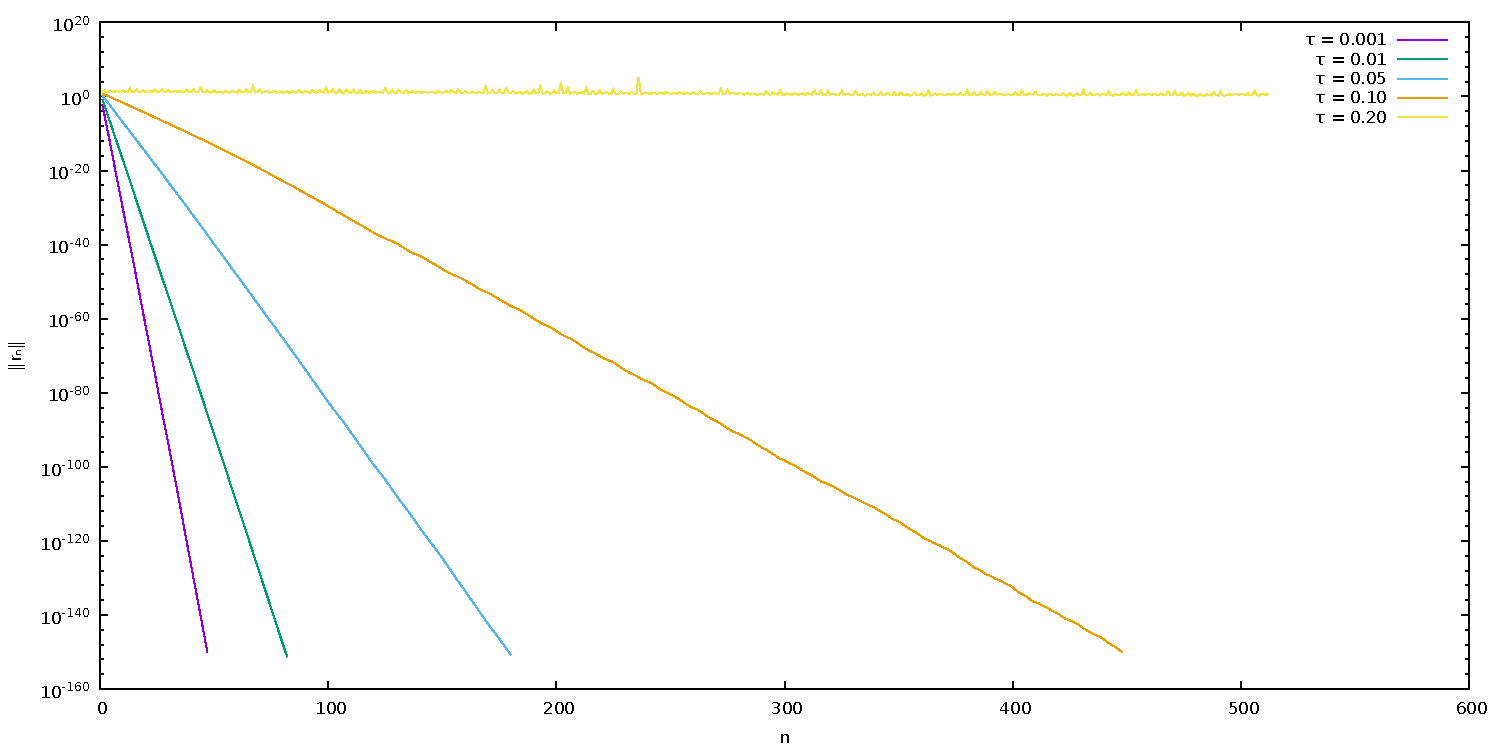
\includegraphics[width=\textwidth]{Exemplos/n_512.pdf}
      \end{figure}

      em que se observa que a taxa de convergência (que pode ser aproximada pela inclinação das retas) cai rapidamente com a densidade da matriz,
      até o caso $\tau = 0.20$, em que a taxa de convergência é nula (linha horizontal). De fato, a matriz em questão não é definida
      positiva e, portanto, o método não tem convergência garantido.

      \newpage
      No entanto, é estranho encontrar resultados na ordem de $10^{-160}$ em algoritmos em geral. Esse número vem de uma raiz quadrada,
      logo antes deveria ser da ordem de $10^{-320}$ o que praticamente o limite \emph{floats} com 64bits ($\approx 10^{-323}$ com números subnormais),
      indicando uma estabilidade impressionante do algoritmo em relação a operações entre valores de ordem similares (evitando \emph{underflow}), uma vez
      que concorda com os resultados do método de Cholesky.

      Podemos inverter a situação e plotar as taxas de convergência para matrizes de diversos tamanhos com a mesma densidade, e obtemos

      \begin{figure}[h]
        \centering
        \caption{Convergências para $\tau = 0.01$}
        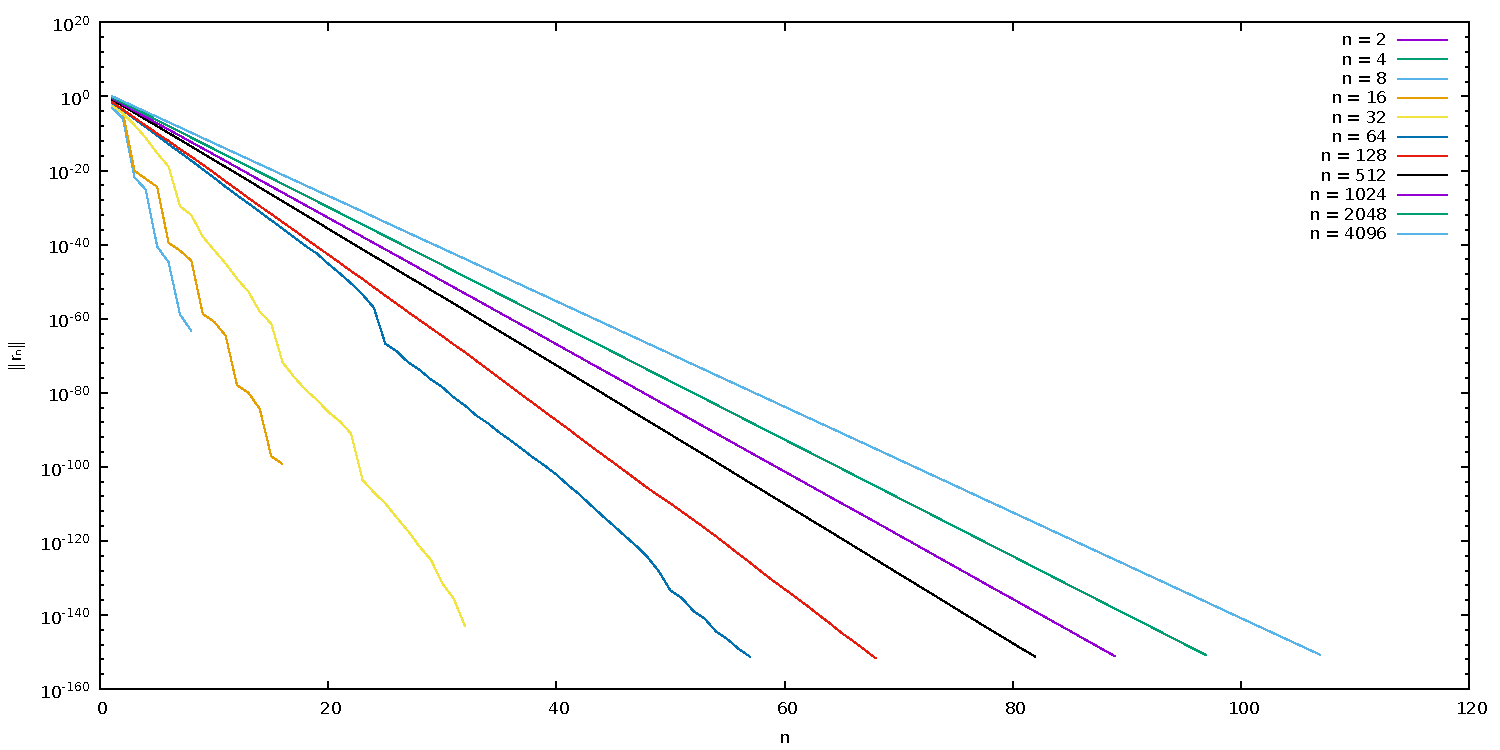
\includegraphics[width=\textwidth]{{Exemplos/tau_0.01}.pdf}
      \end{figure}

      \begin{figure}[h]
        \centering
        \caption{Convergências para $\tau = 0.10$}
        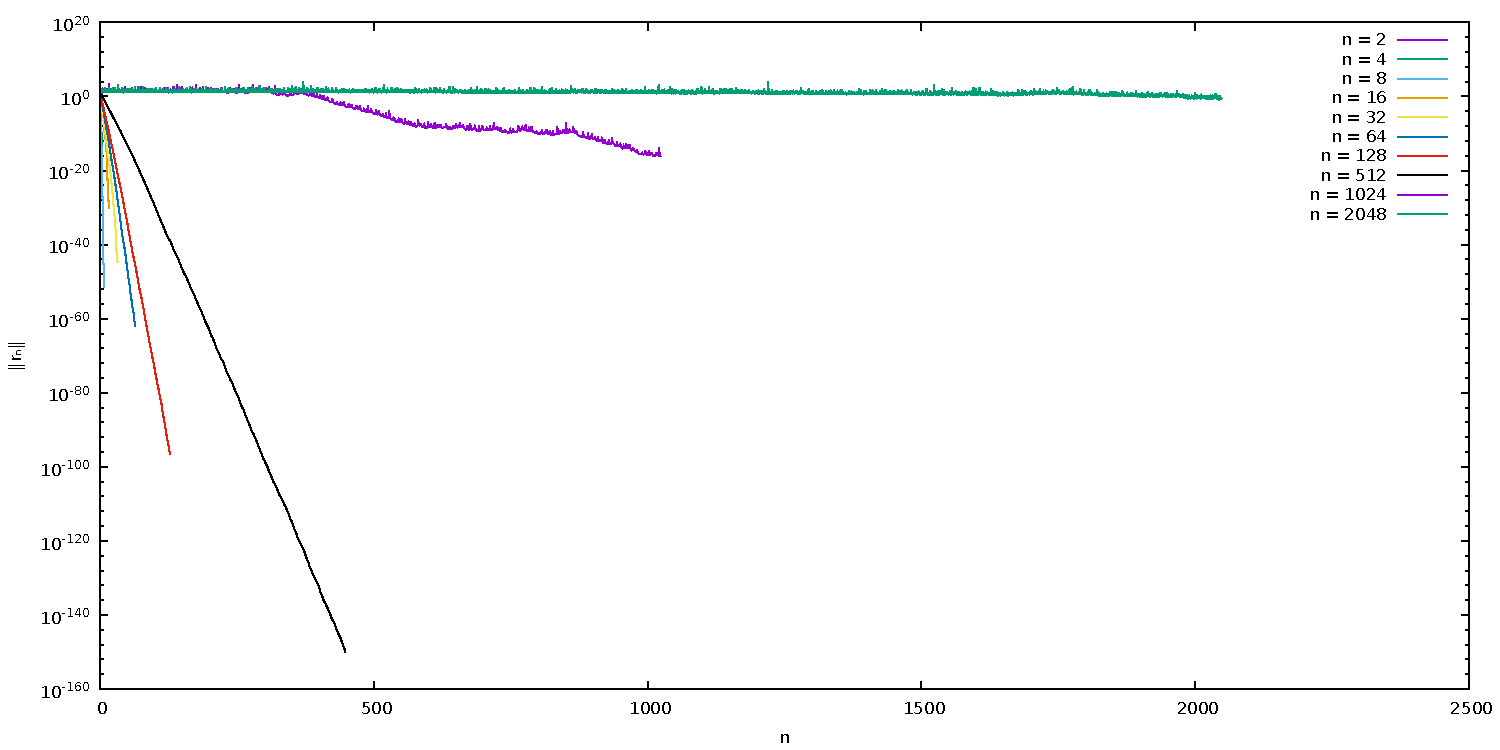
\includegraphics[width=\textwidth]{{Exemplos/tau_0.10}.pdf}
      \end{figure}

      Ambos tipos de gráficos são bem similares, e indicam que a taxa de convergência cai com a densidade e com o tamanho da matriz,
      além de permitir identificar matrizes não definidas positivas.

    \newpage
    \section*{Conclusão}
      Portanto, ao explorar as vantagens apresentadas pelas matrizes esparsas e por ser um algoritmo iterativo de rápida convergência,
      o método de Gradientes Conjugados é o indicado para resolução de sistemas lineares com matrizes de coeficientes grandes, esparsas,
      simétricas e definidas positivas, pois apresenta desempenho ordens de grandeza maior que o método padrão, o de Cholesky.

      A desvantagem é a perda de um método direto para determinar se a matriz é realmente positiva definida, como Cholesky faz,
      mas ainda é possível fazer inferências a partir da taxa de convergência.

      Além disso, seria interessante utilizar um algoritmo de geração de matrizes esparsas aleatórias mais eficiente, que permitisse
      testar matrizes que não coubessem na memória do computador em sua forma densa, já que uma matriz com o maior tamanho testado ainda
      caberia na memória de um computador comum.

    \begin{thebibliography}{9}
        \bibitem{bau97}
            Lloyd N. Trefethen \and David Bau,
            \emph{Numerical Linear Algebra},
            Society for Industrial and Applied Mathematics,
            1997.
    \end{thebibliography}
\end{document}
